\documentclass[a4paper]{report}
\usepackage[utf8]{inputenc}
\usepackage[T1]{fontenc}
\usepackage{RJournal}
\usepackage{amsmath,amssymb,array}
\usepackage{booktabs}


% tightlist command for lists without linebreak
\providecommand{\tightlist}{%
  \setlength{\itemsep}{0pt}\setlength{\parskip}{0pt}}

\usepackage{longtable}

% Always define CSL refs as bib entries are contained in separate doc
% Pandoc citation processing
\newlength{\cslhangindent}
\setlength{\cslhangindent}{1.5em}
\newlength{\csllabelwidth}
\setlength{\csllabelwidth}{3em}
\newlength{\cslentryspacingunit} % times entry-spacing
\setlength{\cslentryspacingunit}{\parskip}
% for Pandoc 2.8 to 2.10.1
\newenvironment{cslreferences}%
  {}%
  {\par}
% For Pandoc 2.11+
\newenvironment{CSLReferences}[2] % #1 hanging-ident, #2 entry spacing
 {% don't indent paragraphs
  \setlength{\parindent}{0pt}
  % turn on hanging indent if param 1 is 1
  \ifodd #1
  \let\oldpar\par
  \def\par{\hangindent=\cslhangindent\oldpar}
  \fi
  % set entry spacing
  \setlength{\parskip}{#2\cslentryspacingunit}
 }%
 {}
\usepackage{calc}
\newcommand{\CSLBlock}[1]{#1\hfill\break}
\newcommand{\CSLLeftMargin}[1]{\parbox[t]{\csllabelwidth}{#1}}
\newcommand{\CSLRightInline}[1]{\parbox[t]{\linewidth - \csllabelwidth}{#1}\break}
\newcommand{\CSLIndent}[1]{\hspace{\cslhangindent}#1}


\usepackage{float, longtable}

\begin{document}


%% do not edit, for illustration only
\sectionhead{Contributed research article}
\volume{16}
\volnumber{4}
\year{2024}
\month{December}
\setcounter{page}{198}

\begin{article}
  % !TeX root = RJwrapper.tex
\title{Changes on CRAN}

\subtitle{%
2024-10-01 to 2024-12-31
}

\author{by Kurt Hornik, Uwe Ligges, and Achim Zeileis}

\maketitle


\hypertarget{cran-growth}{%
\section{CRAN growth}\label{cran-growth}}

In the past 3 months, 504~new packages were
added to the CRAN package repository. 104~packages
were unarchived, 173~were archived and
1~had to be removed. The following shows the
growth of the number of active packages in the CRAN package repository:

\begin{center}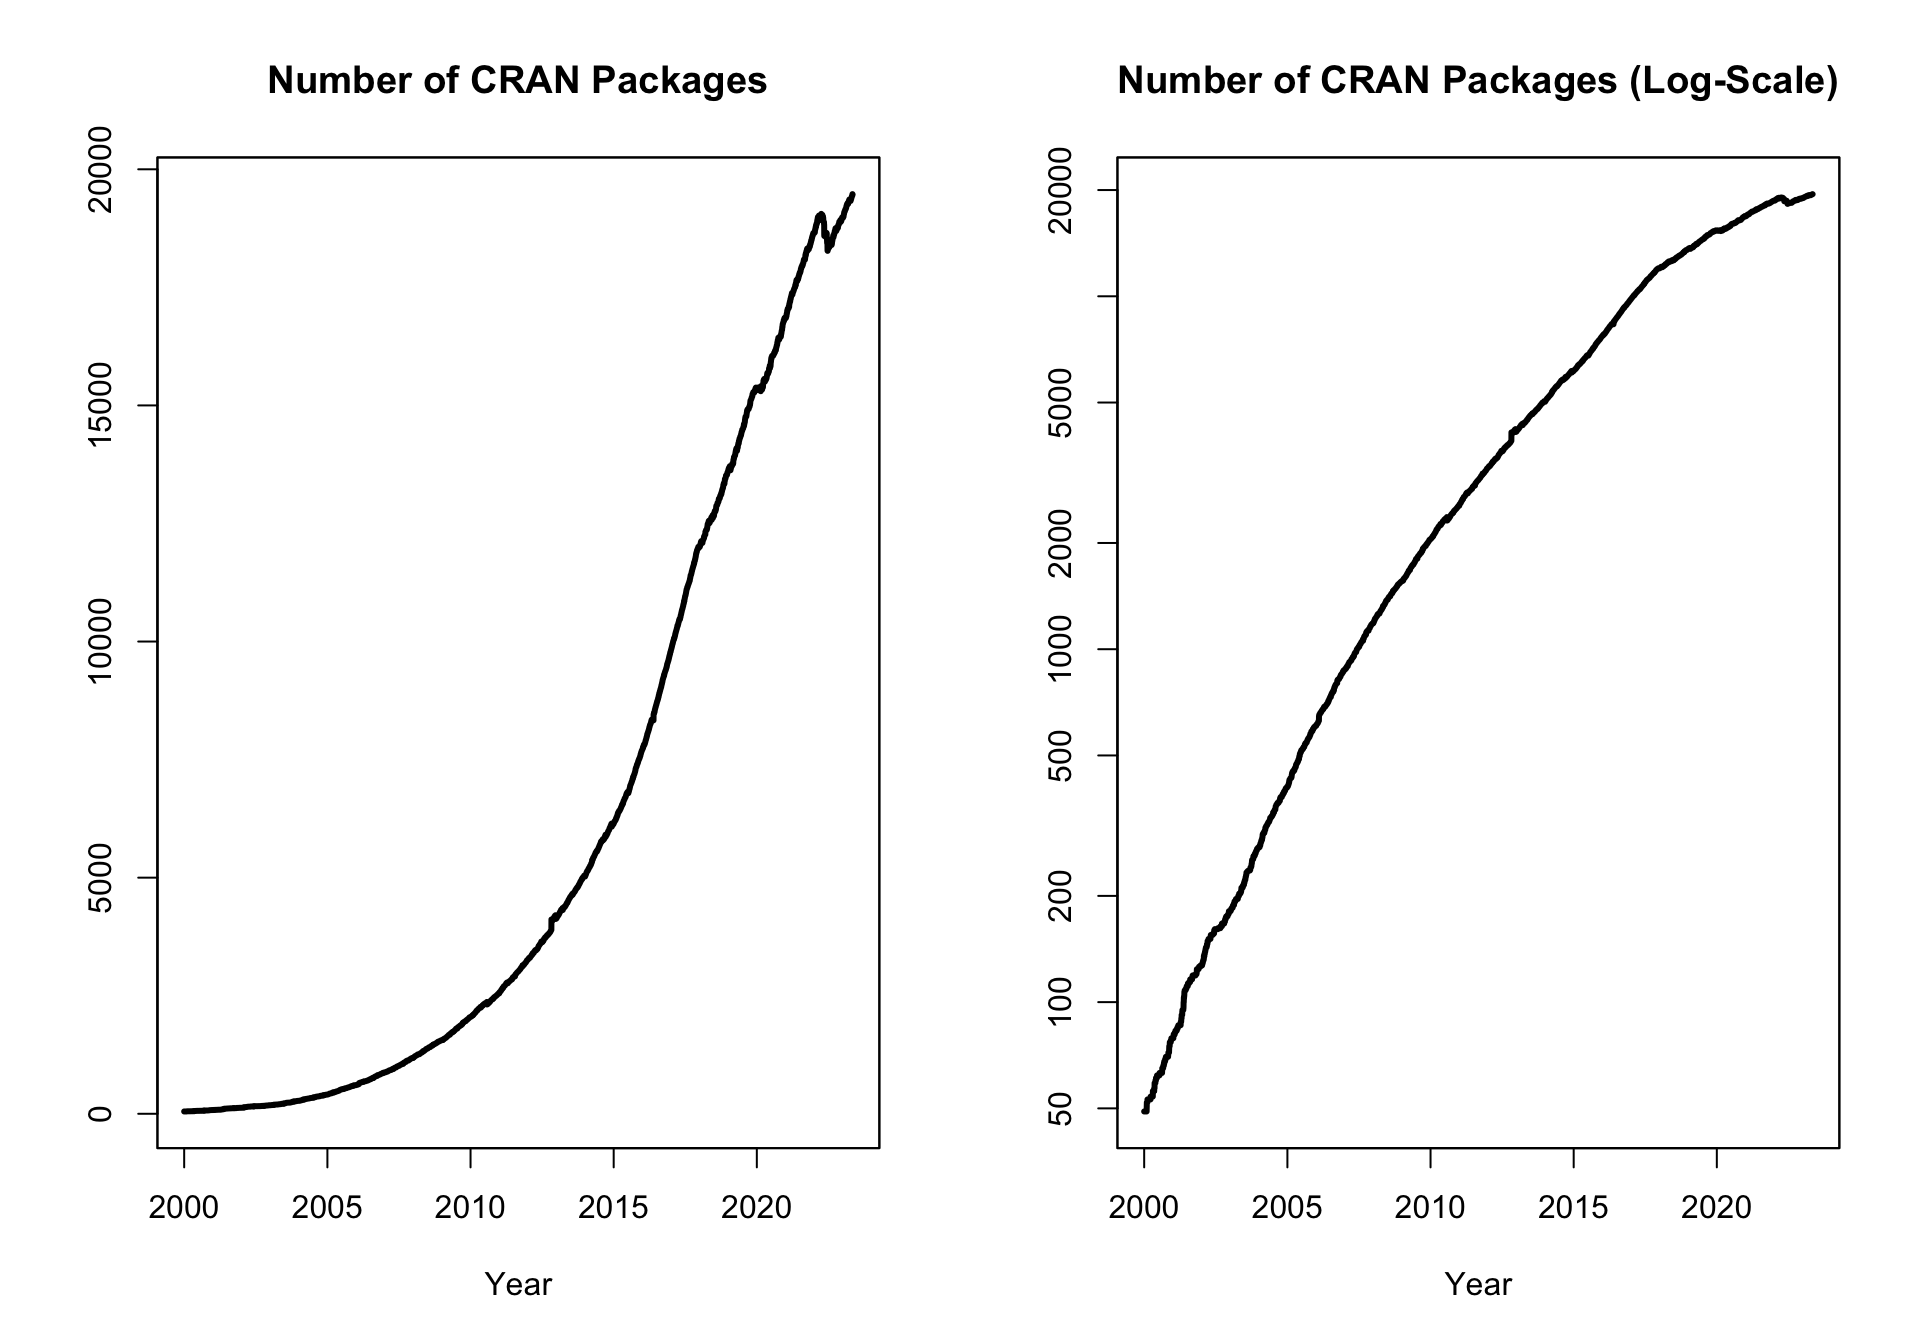
\includegraphics[width=1\linewidth]{RJ-2024-4-cran_files/figure-latex/cran_growth-1} \end{center}

\noindent On 2024-12-31, the number of active packages was around~21860.

\hypertarget{cran-package-submissions}{%
\section{CRAN package submissions}\label{cran-package-submissions}}

From oktober 2024 to december 2024
CRAN received 6179~package submissions.
For these, 9795~actions took place of which
7408~(76\%) were auto processed actions and
2387~(24\%) manual actions.

Minus some special cases, a summary of the auto-processed and manually
triggered actions follows:

\begin{longtable}[]{@{}
  >{\raggedright\arraybackslash}p{(\columnwidth - 16\tabcolsep) * \real{0.0986}}
  >{\raggedleft\arraybackslash}p{(\columnwidth - 16\tabcolsep) * \real{0.1127}}
  >{\raggedleft\arraybackslash}p{(\columnwidth - 16\tabcolsep) * \real{0.1127}}
  >{\raggedleft\arraybackslash}p{(\columnwidth - 16\tabcolsep) * \real{0.1127}}
  >{\raggedleft\arraybackslash}p{(\columnwidth - 16\tabcolsep) * \real{0.1127}}
  >{\raggedleft\arraybackslash}p{(\columnwidth - 16\tabcolsep) * \real{0.1127}}
  >{\raggedleft\arraybackslash}p{(\columnwidth - 16\tabcolsep) * \real{0.1127}}
  >{\raggedleft\arraybackslash}p{(\columnwidth - 16\tabcolsep) * \real{0.1127}}
  >{\raggedleft\arraybackslash}p{(\columnwidth - 16\tabcolsep) * \real{0.1127}}@{}}
\toprule\noalign{}
\begin{minipage}[b]{\linewidth}\raggedright
\end{minipage} & \begin{minipage}[b]{\linewidth}\raggedleft
archive
\end{minipage} & \begin{minipage}[b]{\linewidth}\raggedleft
inspect
\end{minipage} & \begin{minipage}[b]{\linewidth}\raggedleft
newbies
\end{minipage} & \begin{minipage}[b]{\linewidth}\raggedleft
pending
\end{minipage} & \begin{minipage}[b]{\linewidth}\raggedleft
pretest
\end{minipage} & \begin{minipage}[b]{\linewidth}\raggedleft
publish
\end{minipage} & \begin{minipage}[b]{\linewidth}\raggedleft
recheck
\end{minipage} & \begin{minipage}[b]{\linewidth}\raggedleft
waiting
\end{minipage} \\
\midrule\noalign{}
\endhead
\bottomrule\noalign{}
\endlastfoot
auto & 2129 & 490 & 1403 & 96 & 0 & 1991 & 668 & 290 \\
manual & 986 & 0 & 8 & 3 & 27 & 1072 & 226 & 58 \\
\end{longtable}

These include the final decisions for the submissions which were

\begin{longtable}[]{@{}lrr@{}}
\toprule\noalign{}
& archive & publish \\
\midrule\noalign{}
\endhead
\bottomrule\noalign{}
\endlastfoot
auto & 2056 (33.7\%) & 1805 (29.6\%) \\
manual & 982 (16.1\%) & 1254 (20.6\%) \\
\end{longtable}

\noindent where we only count those as \emph{auto} processed whose publication or
rejection happened automatically in all steps.

\hypertarget{cran-mirror-security}{%
\section{CRAN mirror security}\label{cran-mirror-security}}

Currently, there are 94 official CRAN mirrors,
73~of which provide both
secure downloads via `\texttt{https}' \emph{and} use secure mirroring from the CRAN master
(via rsync through ssh tunnels). Since the~R 3.4.0 release, \texttt{chooseCRANmirror()}
offers these mirrors in preference to the others which are not fully secured (yet).

\hypertarget{cran-task-view-initiative}{%
\section{CRAN Task View Initiative}\label{cran-task-view-initiative}}

There is one new task view:

\begin{itemize}
\tightlist
\item
  \href{https://CRAN.R-project.org/view=Paleontology}{Paleontology}: Maintained by William Gearty, Lewis A. Jones, Erin Dillon, Pedro Godoy, Harriet Drage, Christopher Dean, Bruna Farina.
\end{itemize}

Currently there are 48~task views (see \url{https://CRAN.R-project.org/web/views/}),
with median and mean numbers of CRAN packages covered
110 and~121, respectively.
Overall, these task views cover 4885~CRAN packages,
which is about 22\% of all active CRAN packages.


\address{%
Kurt Hornik\\
WU Wirtschaftsuniversität Wien\\%
Austria\\
%
%
\textit{ORCiD: \href{https://orcid.org/0000-0003-4198-9911}{0000-0003-4198-9911}}\\%
\href{mailto:Kurt.Hornik@R-project.org}{\nolinkurl{Kurt.Hornik@R-project.org}}%
}

\address{%
Uwe Ligges\\
TU Dortmund\\%
Germany\\
%
%
\textit{ORCiD: \href{https://orcid.org/0000-0001-5875-6167}{0000-0001-5875-6167}}\\%
\href{mailto:Uwe.Ligges@R-project.org}{\nolinkurl{Uwe.Ligges@R-project.org}}%
}

\address{%
Achim Zeileis\\
Universität Innsbruck\\%
Austria\\
%
%
\textit{ORCiD: \href{https://orcid.org/0000-0003-0918-3766}{0000-0003-0918-3766}}\\%
\href{mailto:Achim.Zeileis@R-project.org}{\nolinkurl{Achim.Zeileis@R-project.org}}%
}

\end{article}


\end{document}
